\section{Λογικά μέρη} \label{section:3-1-logical-parts}

% TODO: discuss the future tense used in this chapter
Η πλατφόρμα χωρίζεται σε δύο λογικά μέρη τα οποία θα αναλυθούν σε λεπτομέρεια στα επόμενα κεφάλαια:

\begin{enumerate}
    \item μία αυτοτελή και πλήρως αποκεντρωτική πλατφόρμα επικοινωνίας γενικής χρήσης
    \item μία μερικώς αποκεντρωτική και μη αυτοτελή επέκταση του πρώτου μέρους στοχευμένη για χρήση από μέλη του ΑΠΘ
\end{enumerate}

\subsection{Πρώτο μέρος} \label{subsection:3-1-first-part}

Το πρώτο μέρος αποτελεί μία αυτοτελή και πλήρως αποκεντρωτική πλατφόρμα. Στόχος της πλατφόρμας είναι να παρέχει τη
δυνατότητα ελευθερίας λόγου, απρόσβλητου σε λογοκρισία από κεντρικές οντότητες εξουσίας. Στην πλατφόρμα αυτή θα μπορεί
οποιοσδήποτε να δημιουργήσει θέματα (topics) ή να απαντήσει σε άλλα. Η επεξεργασία των πληροφοριών που παράγονται και η
οποία είναι αναγκαία για τη λειτουργία της πλατφόρμας θα παρέχεται από το Ethereum μέσω των smart contracts τα οποία θα
υλοποιηθούν στο πλαίσιο αυτής της διπλωματικής. Τα contracts αποτελούν ανοιχτό λογισμικό από τη φύση τους, κάτι το οποίο
ενισχύει την διαφάνεια των διαδικασιών κάνοντας το επιχείρημα της ισότητας του λόγου πιο δυνατό. Τα contracts αυτά θα
δέχονται transactions από τους χρήστες και θα εγγράφουν τα αποτελέσματα στο Storage Layer του blockchain:

\begin{figure}[H]
    \centering
    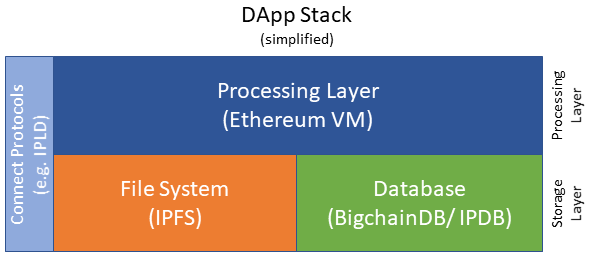
\includegraphics[width=.75\textwidth]{assets/figures/chapter-3/simple_dapp_stack}
    \caption{Ethereum logo}
\end{figure}

Το πρόβλημα αυτής της προσέγγισης είναι πως, για τη λειτουργία της, απαιτείται για κάθε συναλλαγή (transaction) οι
χρήστες να καταβάλουν ένα τέλος. Το τέλος αυτό αφορά τα fees που είναι αναγκαία για την περάτωση των συναλλαγών. Παρόλο
που υπάρχουν σχέδια από την ομάδα ανάπτυξης του Ethereum για τη μείωσή αυτών των fees στο μέλλον, θα είναι πάντα
αναπόφευκτα για τη χρήση του EVM. Ωστόσο, πρέπει να σημειωθούν δύο πράγματα. Αφενός τα τέλη παρέχουν μια μορφή
προστασίας απέναντι σε κακόβουλους χρήστες που θα πλημμύριζαν την εφαρμογή με ανεπιθύμητο ποσοτικά ή ποιοτικά
περιεχόμενο καθώς θα τους ήταν οικονομικά ασύμφορη μια τέτοια επίθεση. Αφετέρου υπάρχουν κάποιες εναλλακτικές ώστε να
μειωθεί δραστικά η εμπλοκή του χρήστη με την καταβολή τελών, κάτι που περιγράφεται παρακάτω στις κατηγορίες χρηστών.

Τα παραπάνω πρακτικά σημαίνουν ότι το Smart Contract θα πρέπει ανά διαστήματα να φορτίζεται με Ether ή οι χρήστες να
καταβάλουν τα δικά τους έξοδα.

\subsection{Δεύτερο μέρος} \label{subsection:3-2-first-part}

Το δεύτερο μέρος αποτελεί μια μερικώς αποκεντρωτική και μη αυτοτελή πλατφόρμα που λειτουργεί προσθετικά στην πρώτη. Το
κομμάτι αυτό απευθύνεται αποκλειστικά σε επικυρωμένα μέλη του ΑΠΘ και συνιστά ένα αμεσοδημοκρατικό σύστημα ψηφοφορίας
που θα εγγυάται σε υψηλό βαθμό την εγκυρότητα και την ανωνυμία των διαδικασιών του. Στο πρώτο μέρος, το οποίο αναλύθηκε
προηγουμένως, θα παρέχεται η δυνατότητα δημιουργίας θεμάτων προς ψηφοφορία. Πάνω στα θέματα αυτά θα ψηφίζουν όσοι έχουν
δικαίωμα, ενώ το δικαίωμα στην ψήφο θα ορίζεται με την κατοχή ενός ανάλογου token στο Ethereum.

\begin{figure}[H]
    \centering
    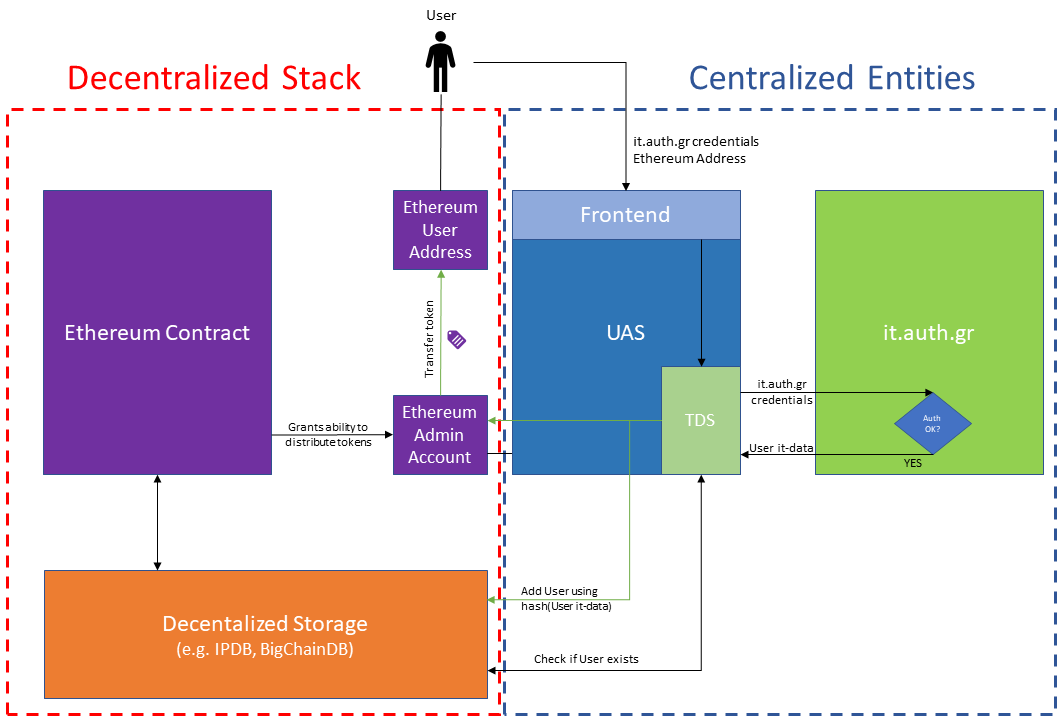
\includegraphics[width=\textwidth]{assets/figures/chapter-3/uas}
    \caption{Ethereum logo}
\end{figure}

O χρήστης, μέσω ενός frontend με τη μορφή ιστοσελίδας, θα μπορεί να πιστοποιήσει μέσω login στο \texttt{it.auth.gr} την
ακαδημαϊκή του ταυτότητα. Στη συνέχεια η Υπηρεσία Διανομής Token (Token Distribution Service - TDS), όντως ο ιδιοκτήτης
(owner) του contract που δινέμει τα tokens θα παρέχει στο χρήστη δύο tokens. Το πρώτο token θα δίνει στον χρήστης το
δικαίωμα ψήφου (verified user token) και το δεύτερο θα σηματοδοτεί στη πλατφόρμα ότι πρέπει του επιστρέφει τα τέλη
(fees) τα οποία πληρώνει (trusted user token).

*Ιδανικά, με τη συνεργασία του ΑΠΘ, το UAS θα αποτελεί υπηρεσία συνεργαζόμενη με την Υποδομή πιστοποίησης και
εξουσιοδότησης (βλ. https://it.auth.gr/el/infrastructure/aai). Αυτό σημαίνει ότι οι χρήστες δε θα χρειάζεται να
εμπιστευτούν τον UAS με τα it credential τους.
